%%%%%%%%%%%%%%%%%%%%%%%%%%%%%%%%%%%%%%%%%%%%%%%%%%%%%%%%%%%%%%%%%%%%%%%%%%%%%%
\section{TS1 collar}

Figure~\ref{figure:vd4_muons_vs_pbars_1037} shows Y:X distribution at VD4 for
muons and antiprotons stopping in the ST.

\begin{figure}[H]
  \begin{tikzpicture}
    \node[anchor=south west,inner sep=0] at (0,0.) {
      % \node[shift={(0 cm,0.cm)},inner sep=0,rotate={90}] at (0,0) {}
      \makebox[\textwidth][c] {
        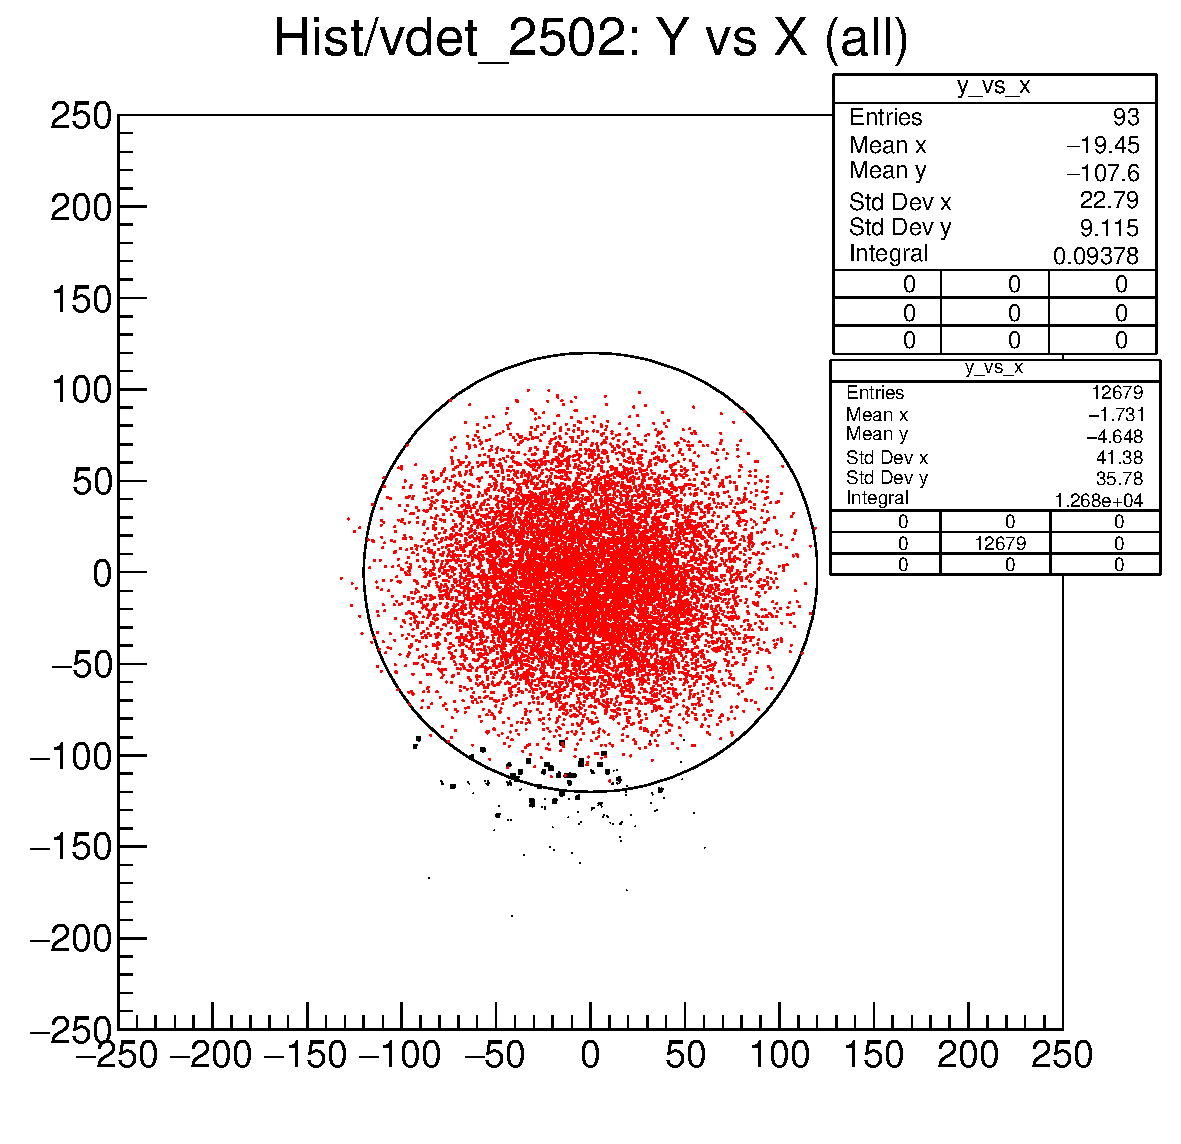
\includegraphics[width=0.5\textwidth]{figures/pdf/vd4_muons_vs_pbars_1037}
      }
    };
    % \node [text width=6cm, scale=0.8] at (4.5,6.4) {mu2e-18894 by Kevin Lynch and Jim Popp};
  \end{tikzpicture}
  \caption{
    \label{figure:vd4_muons_vs_pbars_1037}
    aaa
  }
\end{figure}

%%% Local Variables:
%%% mode: latex
%%% TeX-master: t
%%% End:
